\chapter{Risultati}
\bigskip

\section{Risultati del modello lineare}
\bigskip

Per valutare le performance del modello lineare, oltre all'\textit{errore quadratico medio} abbiamo cercato di misurare con
che precisione il modello tende a predire il picco influenzale, cioè la settimana con la massima incidenza della patologia 
nella popolazione italiana. Come si può notare dalla tabella \ref{tab:linear_model}, nella metà delle stagioni influenzali, 
il modello lineare predice il picco influenzale entro una settimana indicata dai dati InfluNet, inoltre nelle stagioni 
2008-2009, 2011-2012 e 2014-2015 il picco è previsto correttamente). Negli altri quattro casi il modello lineare tende ad 
anticipare la settimana del picco (stagioni 2010-2011, 2013-2014).
\bigskip

Il modello lineare possiede una buona capacità predittiva anche nel caso della stagione influenzale 2009-2010, che fu 
particolarmente grave a causa della diffusione del virus H1N1. Il picco influenzale in questo caso è spostato verso le ultime
settimane del 2009 (dalla numero 42 alla 52) e non corrisponde a l'andamento dei classico della patologia influenzale (si 
nota molto bene da \ref{fig:ch_2_ILI_levels}). Inoltre, quell'anno c'era stata una grande copertura mediatica riguardo 
all'epidemia, cosa che avrebbe potuto in qualche modo aggiungere rumore ai dati del dataset. Nonostante ciò, il modello riesce a prevedere il picco della stagione correttamente (con uno scarto di una settimana).
\bigskip

Abbiamo anche analizzato quale feature siano più importanti per la previsione dei valori di incidenza. Ci siamo soffermati su 
quelle voci di Wikipedia che sono presenti più volte in tutti i modelli e quali di esse avessero il più grande peso 
associato. La tabella \ref{tab:linear_model_feature} mostra le prime 5 feature con peso medio maggiore. Come si può notare, 
sono voci di Wikipedia legate ai sintomi influenzali (inoltre, la voce con più alto peso medio riguarda la patologia 
\textit{Febbre}). Questo sembra confermare la nostra ipotesi iniziale: la popolazione italiana, durante la stagione 
influenzale, naviga su internet alla ricerca di informazioni sull'influenza, in particolare i sintomi. 
\bigskip

Prendendo ad esempio la stagione influenzale 2012-2013, come ci mostra la figura \ref{fig:ch_3_correlation}, si può notare 
come il numero di visite ad alcune voci di Wikipedia inizi ad aumentare esattamente durante il periodo in cui anche 
l'incidenza della patologia influenzale aumenta.
\bigskip

\begin{table}[p]
\centering
\begin{adjustbox}{max width=\textwidth}
\begin{tabular}{|c|c|c|c|c|c|}
\hline
\rowcolor[HTML]{EFEFEF} 
\textbf{Stagione Influenzale} & \textbf{Picco InfluNet (Settimana)} & \textbf{Picco ML (Settimana)} & \textbf{Picco Influnet} & \textbf{Picco ML} & \textbf{MSE}   \\ \hline
\textit{2007-2008}            & \textit{5}                          & \textit{1}                    & \textit{7.21}           & \textit{1.64}     & \textit{11.00} \\ \hline
\rowcolor[HTML]{FFFFFF} 
\textit{2008-2009}            & \textit{4}                          & \textit{4}                    & \textit{8.23}           & \textit{6.64}     & \textit{4.43}  \\ \hline
\rowcolor[HTML]{FFFFFF} 
\textit{2009-2010}            & \textit{46}                         & \textit{45}                   & \textit{12.92}          & \textit{10.89}    & \textit{5.02}  \\ \hline
\rowcolor[HTML]{FFFFFF} 
\textit{2010-2011}            & \textit{5}                          & \textit{4}                    & \textit{11.04}          & \textit{14.80}    & \textit{7.35}  \\ \hline
\rowcolor[HTML]{FFFFFF} 
\textit{2011-2012}            & \textit{5}                          & \textit{5}                    & \textit{9.64}           & \textit{7.99}     & \textit{1.29}  \\ \hline
\rowcolor[HTML]{FFFFFF} 
\textit{2012-2013}            & \textit{6}                          & \textit{5}                    & \textit{9.99}           & \textit{11.95}    & \textit{2.67}  \\ \hline
\rowcolor[HTML]{FFFFFF} 
\textit{2013-2014}            & \textit{6}                          & \textit{3}                    & \textit{6.67}           & \textit{13.80}    & \textit{7.38}  \\ \hline
\rowcolor[HTML]{FFFFFF} 
\textit{2014-2015}            & \textit{4}                          & \textit{4}                    & \textit{10.87}          & \textit{5.11}     & \textit{7.18}  \\ \hline
\rowcolor[HTML]{FFFFFF} 
\textit{2015-2016}            & \textit{8}                          & \textit{5}                    & \textit{6.14}           & \textit{5.59}     & \textit{2.55}  \\ \hline
\end{tabular}
\end{adjustbox}
\caption{\textit{Tabella indicante l'MSE e le varie informazioni sui picchi influenzali nelle varie stagioni. Con la sigla IN si intende il valore indicato dai dati InfluNet, mentre con ML si indica il valore predetto dal modello lineare.}}
\label{tab:linear_model}
\end{table}
\bigskip

\begin{table}[p]
\centering
\begin{adjustbox}{max width=\textwidth}
\begin{tabular}{|l|l|l|}
\hline
\rowcolor[HTML]{EFEFEF} 
\textbf{Feature}                            & \textbf{Peso Medio} & \textbf{Modelli in cui è presente} \\ \hline
\textit{Febbre}                             & \textit{13.11}      & \textit{9/9}                                            \\ \hline
\textit{Influenza}                          & \textit{4.71}       & \textit{9/9}                                            \\ \hline
\textit{Bronchite}                          & \textit{4.64}       & \textit{9/9}                                            \\ \hline
\textit{Influenzavirus\_A\_sottotipo\_H1N1} & \textit{3.98}       & \textit{8/9}                                            \\ \hline
\textit{Polipnea}                           & \textit{3.01}       & \textit{9/9}                                            \\ \hline
\end{tabular}
\end{adjustbox}
\caption{\textit{Tabella indicante le prime 5 feature ordinate per il loro peso medio e in quanti modelli essi compaiano.}}
\label{tab:linear_model_feature}
\end{table}

\begin{figure}[p]
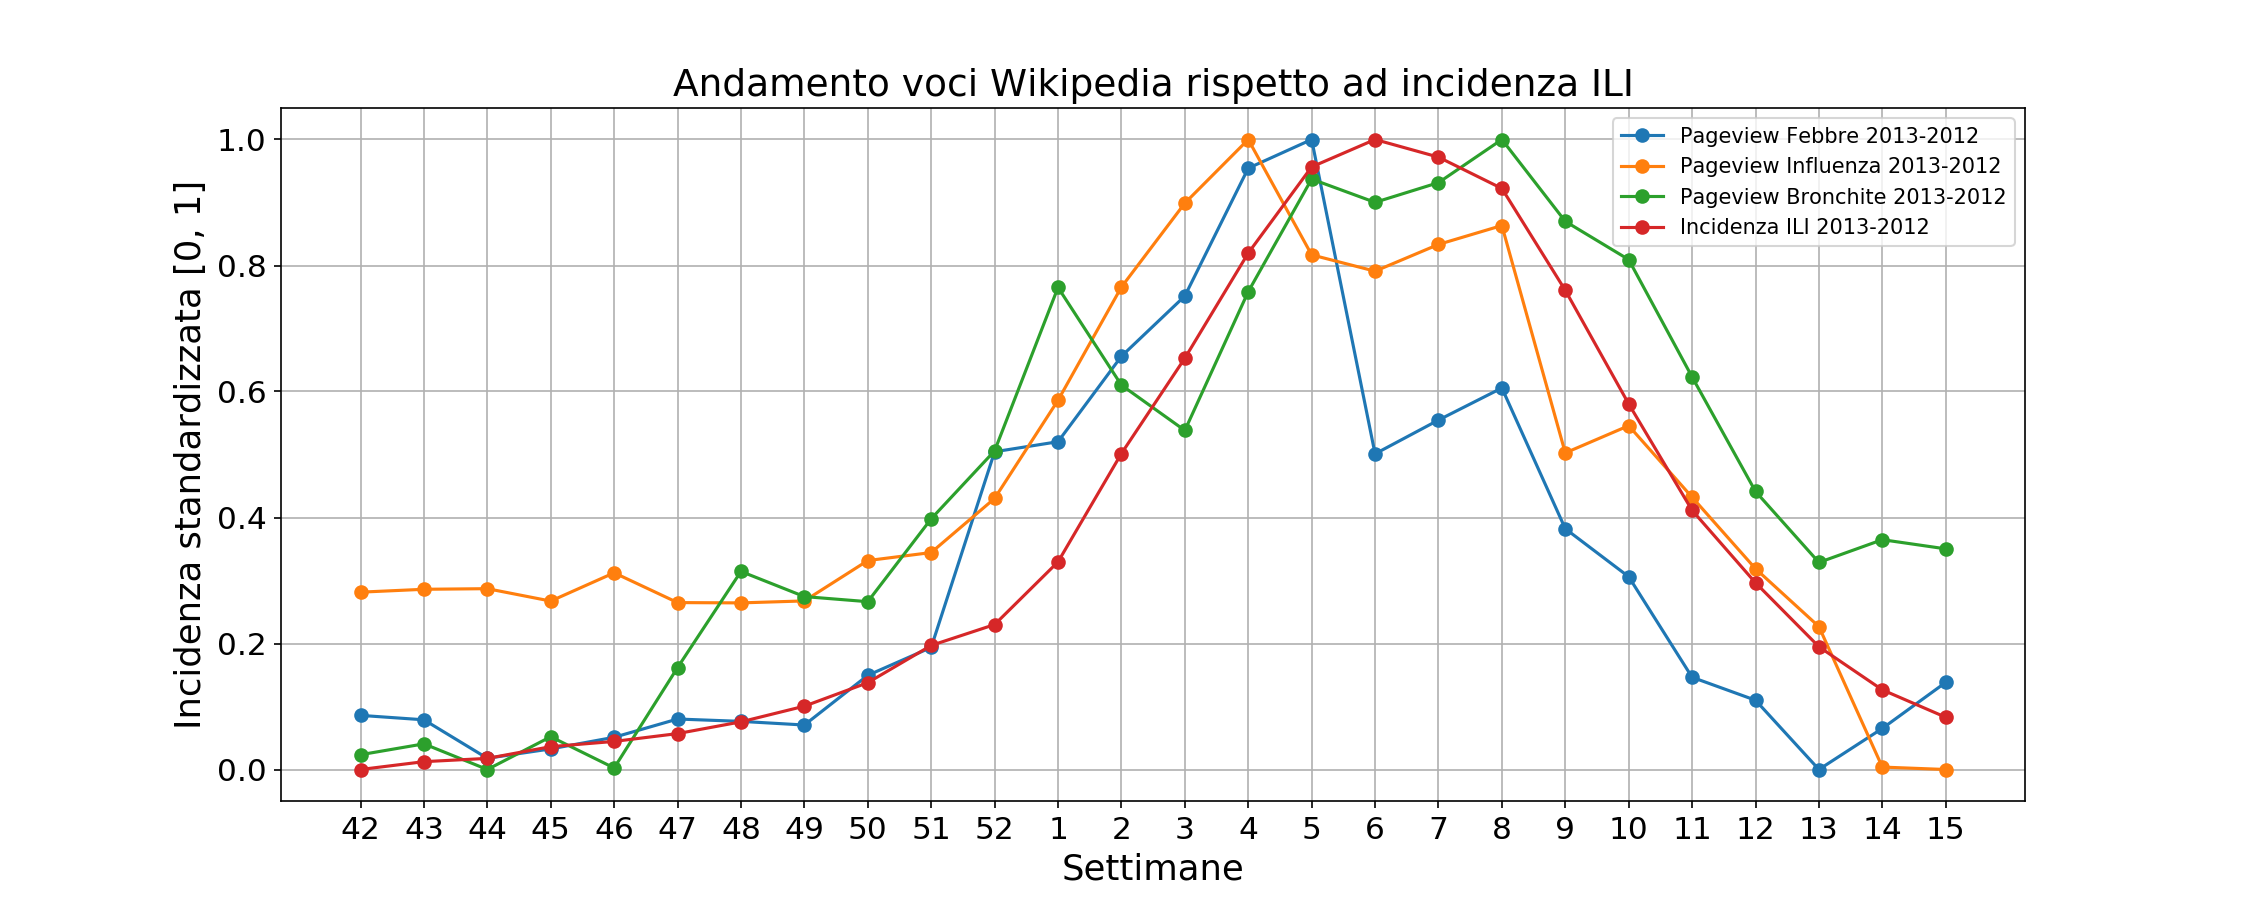
\includegraphics[width=\textwidth]{chapter_3_correlation}
\caption{\textit{Variazione del valore di alcune feature rispetto all'incidenza ILI (i valori per essere comparati sono stati normalizzati nell'intervallo [0,1]).}}
\label{fig:ch_3_correlation}
\centering
\end{figure}

\section{Risultati del modello di Poisson}

Nonostante nel paper di riferimento l'utilizzo di un modello generalizzato si sia rivelato efficiente e adatto a stimare i livelli di ILI negli Stati Uniti, per l'Italia il modello di Poisson non ha mostrato significativi miglioramenti rispetto al modello lineare, anzi in certi casi ha mostrato un significativo calo di prestazioni. Come mostra la tabella \ref{tab:ch_3_poisson_model}, pur riuscendo a stimare il picco influenzale (con uno scarto di una settimana) in cinque stagioni su nove, in alcuni casi il modello sovrastima in maniera abbondante l'incidenza del picco. Ad esempio, nella stagione influenzale 2009-2010 la sovrastima è particolarmente evidente.
\bigskip

Riguardo alle feature utilizzate, osservando la tabella \ref{tab:ch_3_poisson_model_feature}, si nota come il modello di Poisson tenda a dare maggior peso a voci di Wikipedia che poco anno a che fare con i sintomi della patologia influenzale. Inoltre, i pesi assegnati hanno un entità molto minore rispetto a quelli del modello lineare. Osservando inoltre l'andamento delle feature rispetto al valore dell'incidenza ILI si può notare come non ci sia una corrispondenza così netta come nel caso del modello lineare (figura \ref{fig:ch_3_correlation_poisson}).
\bigskip

\section{Conclusioni}

\begin{table}[p]
\centering 
\begin{adjustbox}{max width=\textwidth}
\begin{tabular}{|c|c|c|c|c|c|}
\hline
\rowcolor[HTML]{EFEFEF} 
\textbf{Stagione Influenzale} & \textbf{Picco InfluNet (Settimana)} & \textbf{Picco ML (Settimana)} & \textbf{Picco Influnet} & \textbf{Picco ML} & \textbf{MSE}      \\ \hline
\textit{2007-2008}            & \textit{5}                          & \textit{1}                    & \textit{7.21}           & \textit{1.01}     & \textit{13.02}    \\ \hline
\rowcolor[HTML]{FFFFFF} 
\textit{2008-2009}            & \textit{4}                          & \textit{4}                    & \textit{8.23}           & \textit{5.78}     & \textit{3.31}     \\ \hline
\rowcolor[HTML]{FFFFFF} 
\textit{2009-2010}            & \textit{46}                         & \textit{45}                   & \textit{12.92}          & \textit{1090.86}  & \textit{44764.56} \\ \hline
\rowcolor[HTML]{FFFFFF} 
\textit{2010-2011}            & \textit{5}                          & \textit{6}                    & \textit{11.04}          & \textit{59.16}    & \textit{147.97}   \\ \hline
\rowcolor[HTML]{FFFFFF} 
\textit{2011-2012}            & \textit{5}                          & \textit{5}                    & \textit{9.64}           & \textit{8.57}     & \textit{1.27}     \\ \hline
\rowcolor[HTML]{FFFFFF} 
\textit{2012-2013}            & \textit{6}                          & \textit{8}                    & \textit{9.99}           & \textit{8.45}     & \textit{6.25}     \\ \hline
\rowcolor[HTML]{FFFFFF} 
\textit{2013-2014}            & \textit{6}                          & \textit{3}                    & \textit{6.67}           & \textit{16.48}    & \textit{6.15}     \\ \hline
\rowcolor[HTML]{FFFFFF} 
\textit{2014-2015}            & \textit{4}                          & \textit{5}                    & \textit{10.87}          & \textit{4.95}     & \textit{9.73}     \\ \hline
\rowcolor[HTML]{FFFFFF} 
\textit{2015-2016}            & \textit{8}                          & \textit{7}                    & \textit{6.14}           & \textit{5.23}     & \textit{2.64}     \\ \hline
\end{tabular}
\end{adjustbox}
\caption{\textit{Tabella indicante l'MSE e le varie informazioni sui picchi influenzali nelle varie stagioni. Con la sigla IN si intende il valore indicato dai dati InfluNet, mentre con ML si indica il valore predetto dal modello lineare.}}
\label{tab:ch_3_poisson_model}
\end{table}

\begin{table}[p]
\centering 
\begin{adjustbox}{max width=\textwidth}
\begin{tabular}{|l|l|l|}
\hline
\rowcolor[HTML]{C0C0C0} 
{\color[HTML]{000000} \textbf{Feature}}         & {\color[HTML]{000000} \textbf{Peso Medio}} & {\color[HTML]{000000} \textbf{Modelli in cui è presente}} \\ \hline
\textit{Pagina principale}                      & \textit{0.52}                              & \textit{9/9}                                              \\ \hline
\textit{Febbre ricorrente}                      & \textit{0.07}                              & \textit{9/9}                                              \\ \hline
\textit{Vaccino per la febbre tifoide}          & \textit{0.06}                              & \textit{2/9}                                              \\ \hline
\textit{Stimmate\_(medicina)}                   & \textit{0.05}                              & \textit{8/9}                                              \\ \hline
\textit{Virus dell'encefalite di Murray Valley} & \textit{0.05}                              & \textit{2/9}                                              \\ \hline
\end{tabular}
\end{adjustbox}
\caption{\textit{Tabella indicante l'MSE e le varie informazioni sui picchi influenzali nelle varie stagioni. Con la sigla IN si intende il valore indicato dai dati InfluNet, mentre con ML si indica il valore predetto dal modello lineare.}}
\label{tab:ch_3_poisson_model_feature}
\end{table}

\begin{figure}[p]
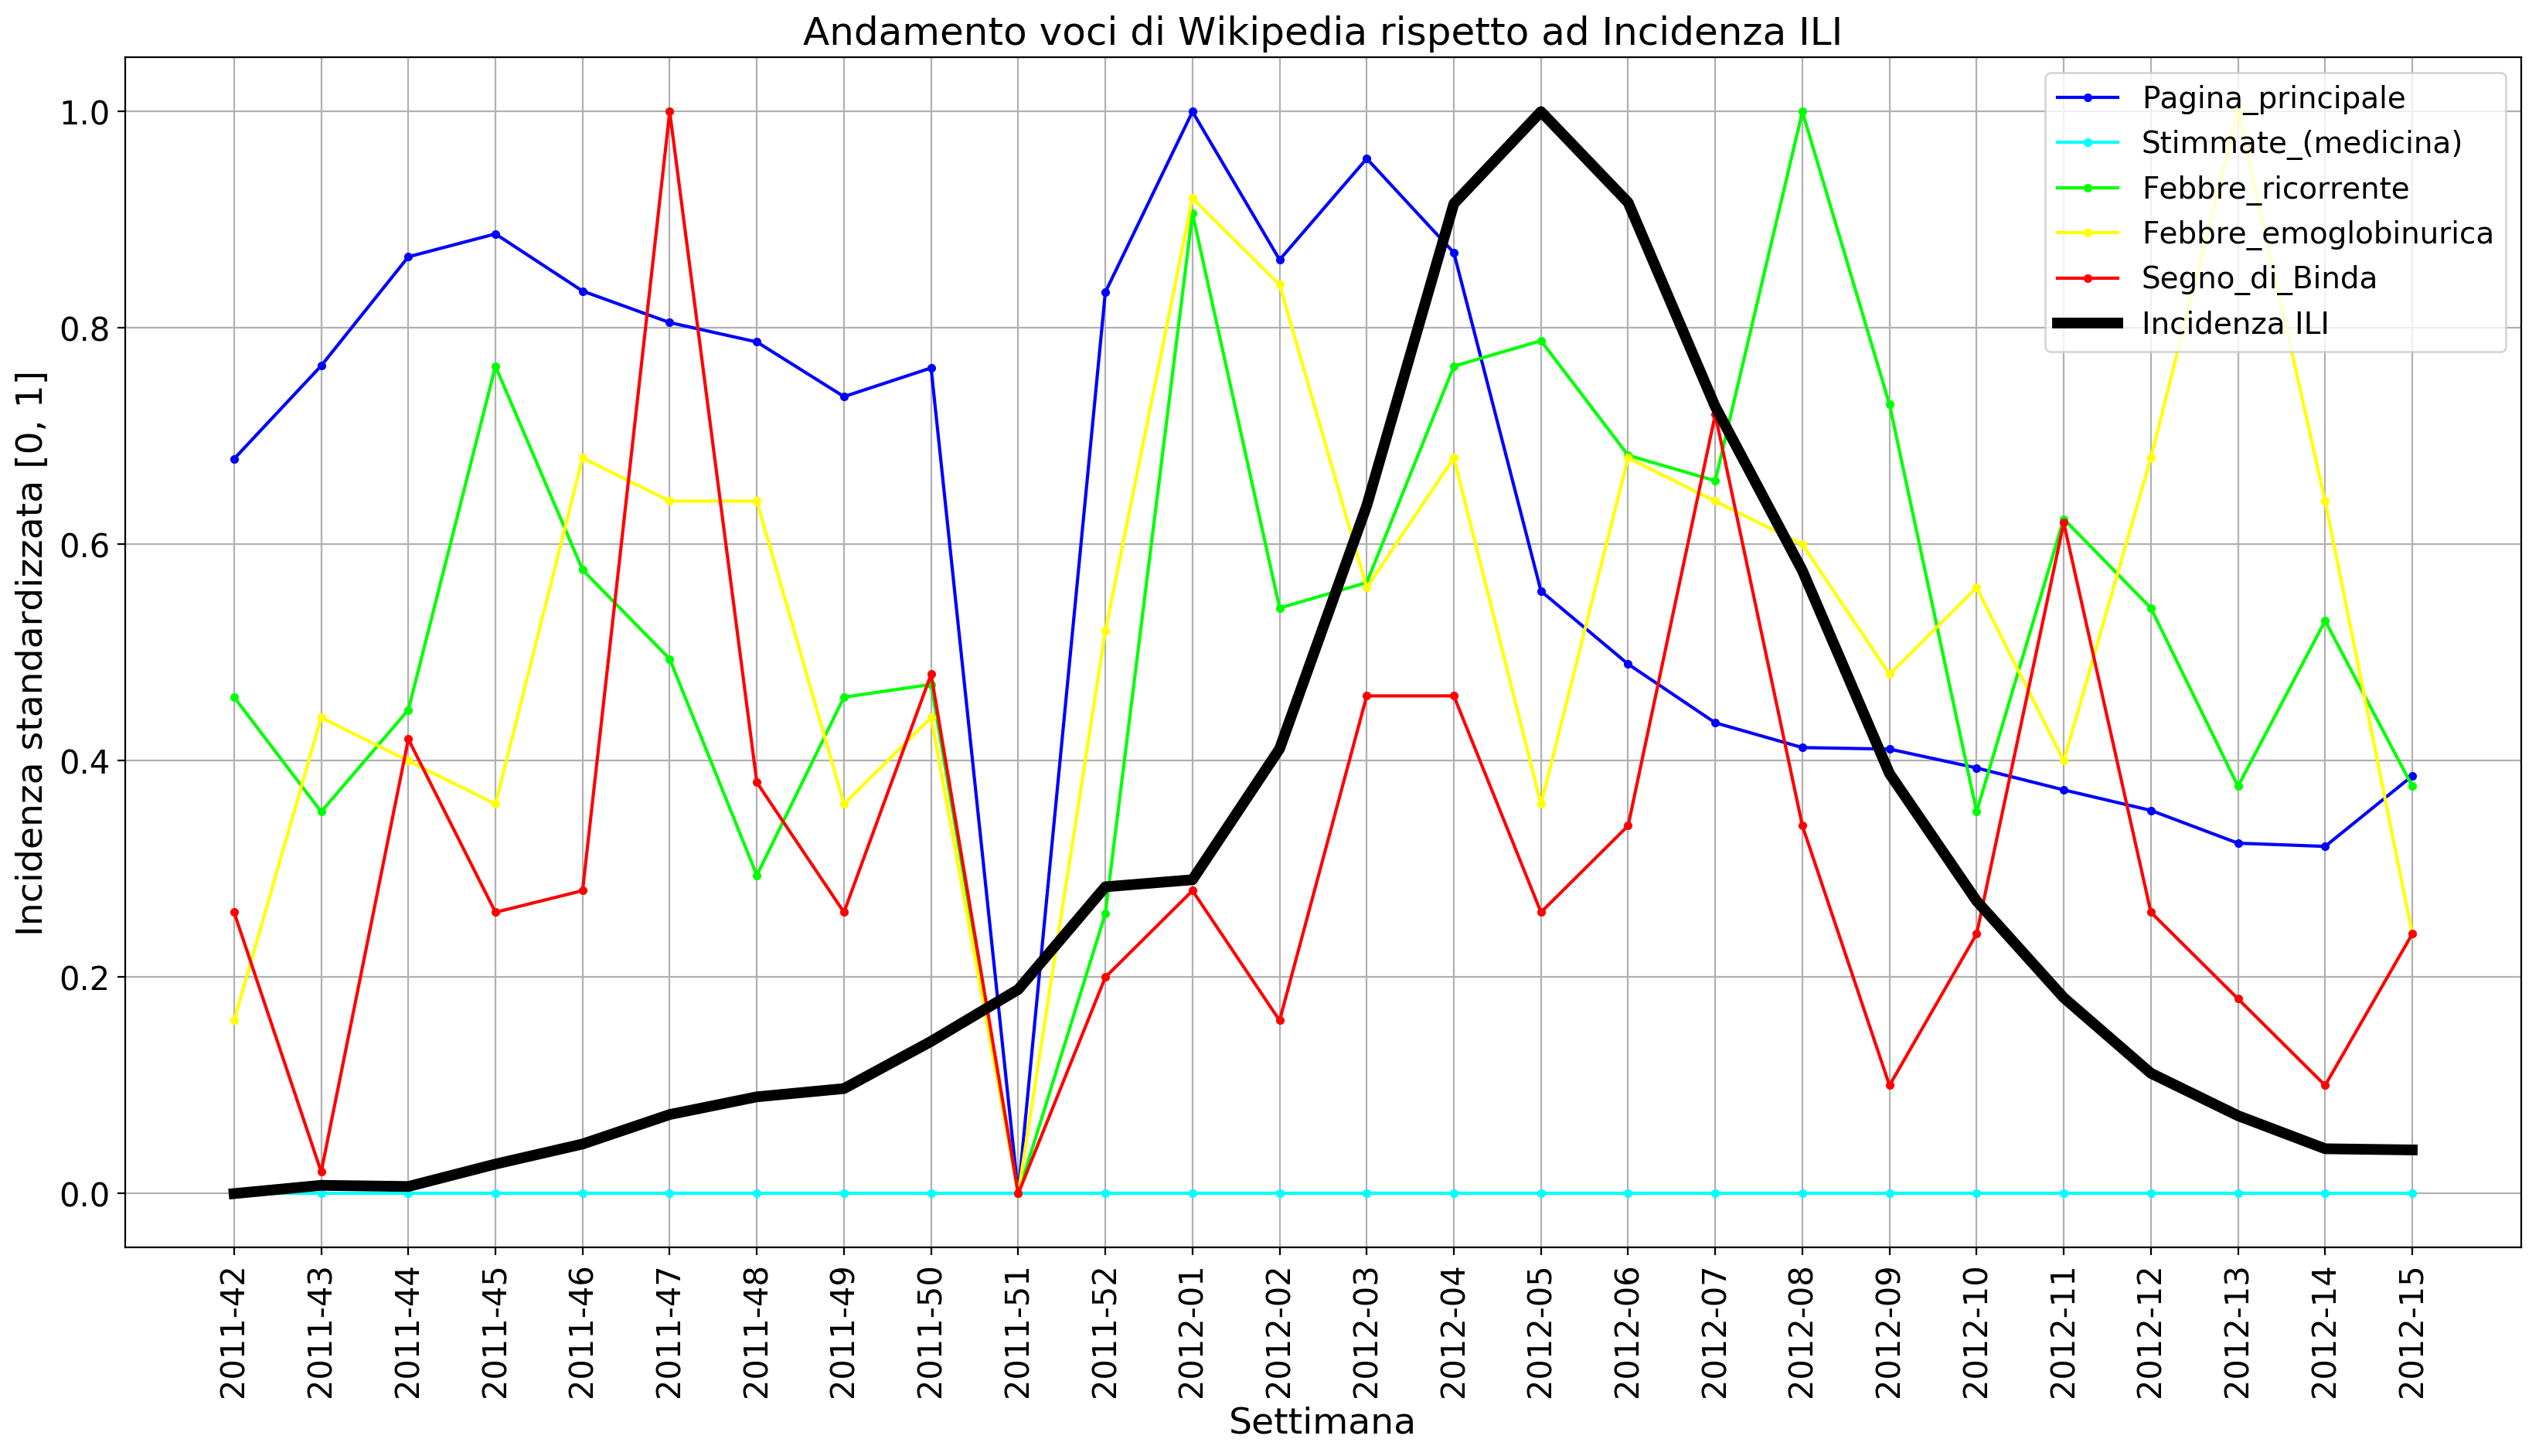
\includegraphics[width=\textwidth]{chapter_3_correlation_poisson}
\caption{\textit{Variazione del valore delle prime 5 feature rispetto all'incidenza ILI (i valori per essere comparati sono stati normalizzati nell'intervallo [0,1]).}}
\label{fig:ch_3_correlation_poisson}
\centering
\end{figure}